\problem{Кристаллохимия}{10}

\ProblemPointsSeven{4}{4}{6}{4}{4}{10}{8}{40}{10}

При взаимодействии металла \em{А} с неметаллом \em{Б} можно получить вещества \em{В} или \em{Г}, которые могут применяться как полупроводники и вещества, поглощающие микроволновое излучение.

Также синтез можно провести в гидротермальном реакторе при температурах выше 100\unit{\celsius}. Для этого смешивают водный раствор вещества \em{Д} с раствором, полученным растворением \em{Б} в растворе $\ce{NaOH}$ (\em{реакция 1}), затем добавляют к смеси гидразин ($\ce{N2H4}$) и нагревают в закрытой бомбе. В этой смеси при температурах 100-120\unit{\celsius} образуется чистый \em{Г} (\em{реакция 2}), а при температуре 180\unit{\celsius} через 6 часов кипячения образуется чистый \em{В} (\em{реакция 3}). \em{Реакции 2} и \em{3} протекают сложно: в них гидразин играет роль восстановителя, один из продуктов \em{реакции 1} --- роль окислителя, а \em{Д} --- источник металла \em{А}. Известен массовый состав вещества \em{Д}.

\begin{table}[H]
  \centering
  \begin{tabularx}{0.8\textwidth}{|Y|Y|Y|Y|}
    \hline
    $\omega (\mathbf{A})$ & $\omega (\mathbf{C})$ & $\omega (\mathbf{O})$ & $\omega (\mathbf{H})$ \\
    \hline
    26.28\% & 22.98\% & 45.92\% & 4.82\% \\
    \hline
  \end{tabularx}
\end{table}

На рисунках 1 и 2.\textit{а} показаны элементарные ячейки кристаллических решеток \em{В} и \em{Г}, соответственно. На рисунке 2.\textit{б} показан также вид сверху, совпадающий с видом спереди и сбоку, на ячейку \em{Г}. Сиреневые атомы --- \em{А}, оранжевые --- \em{Б}.

\begin{figure}[H]
  \centering
  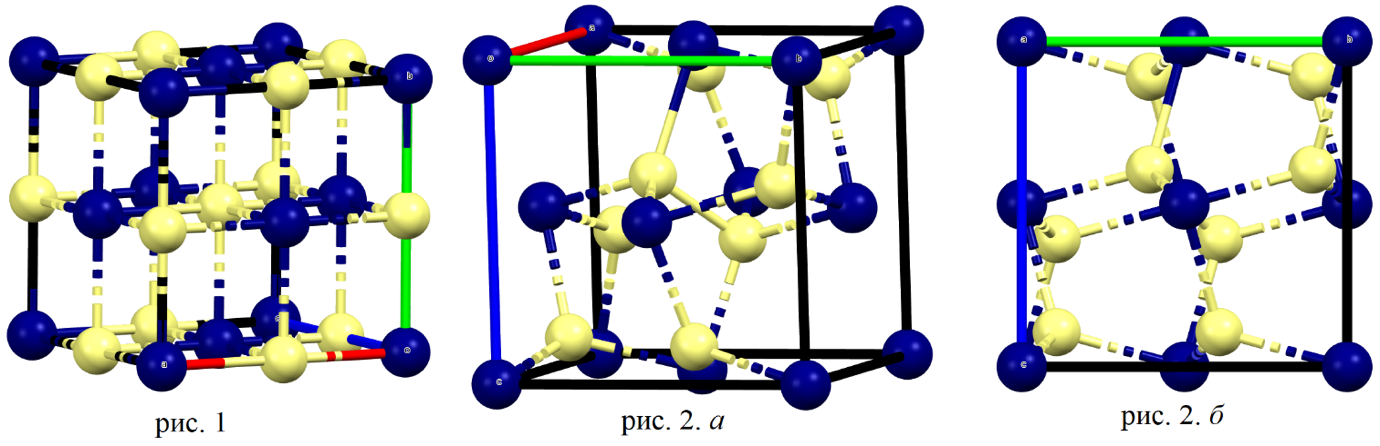
\includegraphics[width=\textwidth]{problems/problem4/images/image1}
\end{figure}

\begin{enumerate}
  \item Сколько атомов \em{А} и атомов \em{Б} расположено в одной элементарной ячейке вещества \em{В}? вещества \em{Г}?
  \item Каково координационное число \em{А} в веществе \em{В}? в веществе \em{Г}?
  \item Используя плотности и параметр ячеек \em{В} и \em{Г}, определите молярные массы элементов \em{А} и \em{Б}, запишите формулы \em{В} и \em{Г} и укажите степени окисления элементов в них.

  \begin{table}[H]
    \centering
    \begin{tabularx}{0.7\textwidth}{|Y|Y|Y|}
      \hline
       & $a,$ \unit{\angstrom} & $\rho,$ \unit{\gram\per\centi\meter\cubed} \\
      \hline
      \em{В} & 5.440 & 5.52 \\
      \hline
      \em{Г} & 6.417 & 5.35 \\
      \hline
    \end{tabularx}
  \end{table}

  \item Какова электронная конфигурация металла \em{А} в \em{В}? Приведите пример еще одного элемента в устойчивой степени окисления с такой же электронной конфигурацией.

  \item Приведите пример хотя бы одного природного вещества, изоструктурного \em{В}, и хотя бы одного природного вещества, изоструктурного \em{Г}.

  \item Определите формулу вещества \em{Д} и напишите уравнения \em{реакций 1--3}.
\end{enumerate}

\begin{minipage}{\textwidth}
  \begin{minipage}{0.6\textwidth}
    \begin{enumerate}
      \setcounter{enumi}{6}
      \item Подробное рассмотрение структуры \em{Г} показывает, что 2 атома \em{Б} (на рис. 3 помечены \textit{a} и \textit{b}) расположены на диагонали куба и равноудалены от вершин куба, образующих её концы. Известно, что расстояние от атома $a$ до ближайшего атома элемента \em{А} (помечен \textit{с}) составляет 2.379\unit{\angstrom}, а угол \textit{dac} при атоме a равен 75.8\unit{\degree}.

      Рассчитайте длину связи \em{Б-Б} (то есть расстояние \textit{ab}) в веществе \em{Г}.
    \end{enumerate}
  \end{minipage}
  \hspace{0.05\textwidth}
  \begin{minipage}{0.3\textwidth}
    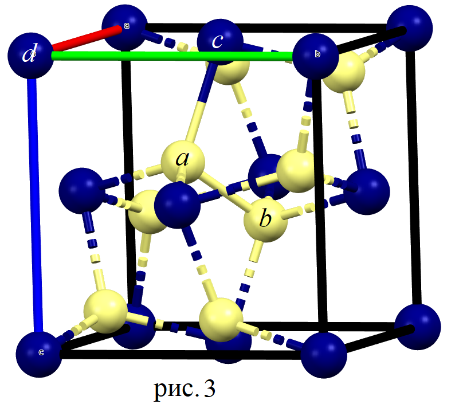
\includegraphics[width=\textwidth]{problems/problem4/images/image2}
  \end{minipage}
\end{minipage}